% Included from both -slides and -handout versions.
%
% TODO:
%
% A page-table + TLB picture would go a long way to explaining how the
% software view starts to map into hardware.
%
% A copy-on-write picture would be good.
%
% Shift slide introducing traps to the following lecture.

\mode<presentation>
{
  \usetheme{default}
  \useoutertheme{infolines}
}

\usepackage[english]{babel}
\usepackage[latin1]{inputenc}
\usepackage{graphicx}
\usepackage{times}
\usepackage[T1]{fontenc}
\usepackage{fancyvrb}
\usepackage{listings}
\begin{document}
\lstset{language=C, escapeinside={(*@}{@*)}, numbers=left,
  basicstyle=\tiny, showspaces=false, showtabs=false}

\title{L41 - Lecture 3: The Process Model (1)}
%\institute{University of Cambridge}
%\author{George V. Neville-Neil}
\author{Dr Robert N. M. Watson}
\date{2 November 2015}

\begin{frame}
  \titlepage
\end{frame}

\section{Introduction}

\begin{frame}
  \frametitle{Reminder: last time}

  \begin{enumerate}
    \item DTrace
    \item The probe effect
    \item The kernel source
    \item A little on kernel dynamics
  \end{enumerate}
\end{frame}

\section{The Process Model}

\begin{frame}
  \frametitle{This time: the process model}

  \begin{enumerate}
    \item The process model and its evolution
    \item Brutal (re,pre)-introduction to virtual memory
    \item Where do programs come from?
    \item Traps and system calls
    \item Reading for next time
  \end{enumerate}
\end{frame}

\begin{frame}
  \frametitle{The process model: 1970s foundations}
  \begin{columns}[T]
    \column{0.4\textwidth}
      \vspace{1.25cm}
      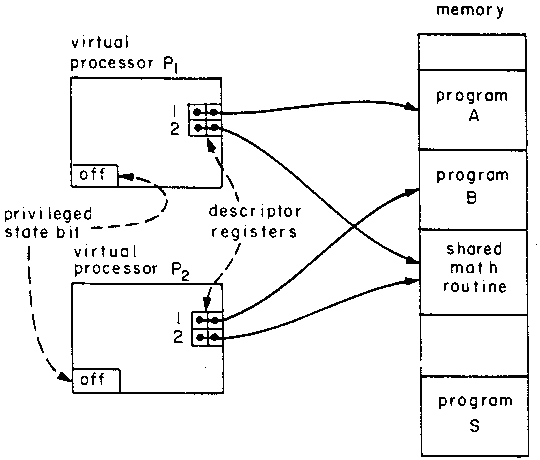
\includegraphics[width=1.1\textwidth]{../../figures/saltzer-schroeder-protection.png}

    \column{0.5\textwidth}
      \begin{itemize}
	\item Saltzer and Schroeder, \textit{The Protection of Information in
	  Computer Systems}, SOSP'73, October 1973.
	  (CACM 1974)

	\pause

	\item \textit{Multics} process model
	\begin{itemize}
	  \item `Program in execution'
	  \item \textit{Process isolation} bridged by \textit{controlled
	  communication} via supervisor (kernel)
	\end{itemize}

	\pause

	\item Hardware foundations
	\begin{itemize}
	  \item Supervisor mode
	  \item Memory segmentation
	  \item Trap mechanism
	\end{itemize}

	\pause

	\item Hardware protection rings (Schroeder and Saltzer, 1972)
      \end{itemize}
  \end{columns}
\end{frame}

\begin{frame}
  \frametitle{The process model: today}

  \begin{columns}[T]
    \column{0.45\textwidth}
      \vspace{0.5cm}
      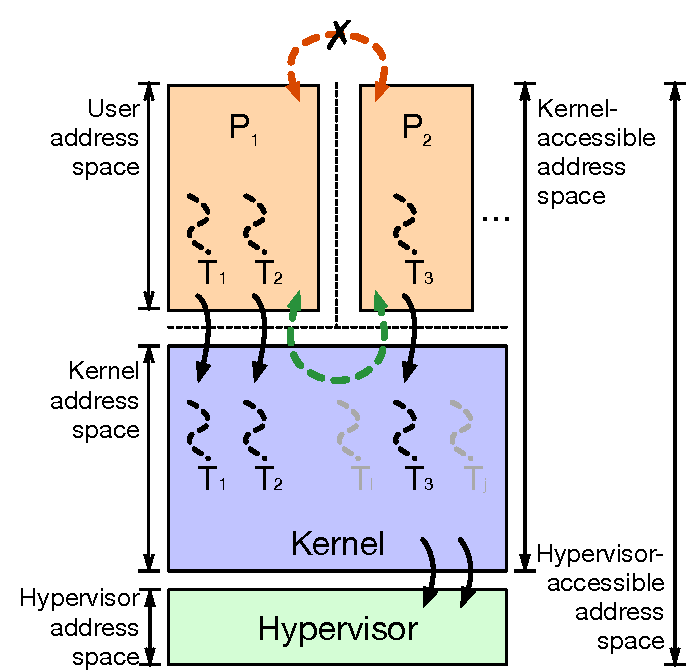
\includegraphics[width=1.1\textwidth]{../../figures/kernel-user-threads.pdf}

    \column{0.5\textwidth}
      % Explain the diagram has rotated sideway!
      \pause

      \begin{itemize}
        \item `Program in execution'
	\begin{itemize}
	  \item Process $\approx$ address space
          \item `Threads' execute code
	\end{itemize}


	\pause

	\item Unit of resource accounting
	\begin{itemize}
	  \item Open files, memory, ...
	\end{itemize}

	\pause

        \item Kernel interaction via \textit{traps}: \\
	  system calls, page faults, ...

	\pause

	\item Hardware foundations
	\begin{itemize}
	  \item Rings control MMU, I/O, etc.
	  \item Virtual addressing (MMU)
	  \item Trap mechanism
        \end{itemize}

        \pause

	\item Details vary little across \{BSD, OS~X, Linux, Windows, ...\}

	\pause

	\item Recently: OS-App trust model inverted: Trustzone, SGX
      \end{itemize}
  \end{columns}
\end{frame}

\begin{frame}
  \frametitle{The UNIX process life cycle}

  \begin{columns}[T]
    \column{0.5\textwidth}
      \vspace{0.5cm}
      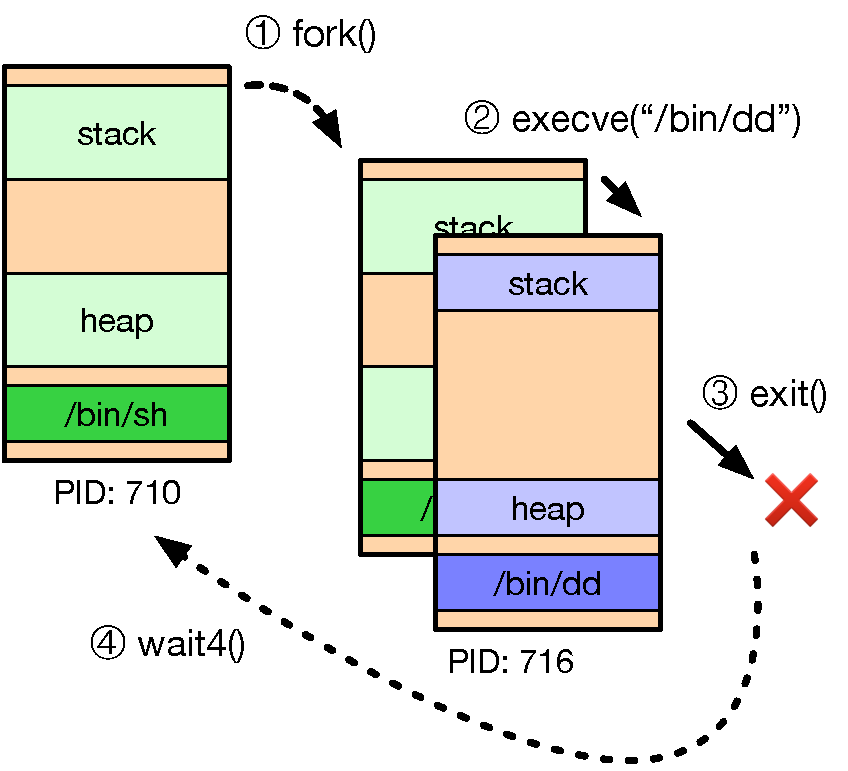
\includegraphics[width=\textwidth]{../../figures/process-life-cycle.pdf}

    \column{0.5\textwidth}
    \begin{itemize}

      \pause

      \item \texttt{fork()}
      \begin{itemize}
	\item Child inherits address space and other properties
	\item Program prepares process for new binary (e.g., \texttt{stdio})
	\item Copy-on-Write (COW)
      \end{itemize}

      \pause

      \item \texttt{execve()}
      \begin{itemize}
	\item Kernel replaces address space, loads new binary, starts execution
      \end{itemize}

      \pause

      \item \texttt{exit()}
      \begin{itemize}
	\item Process can terminate self (or be terminated)
      \end{itemize}

      \pause

      \item \texttt{wait4} (et al)
      \begin{itemize}
	\item Parent can await exit status
      \end{itemize}
    \end{itemize}
  \end{columns}
\end{frame}

\begin{frame}
  \frametitle{Process model evolution}

  \begin{columns}[T]
    \column{0.5\textwidth}
      \vspace{1cm}
      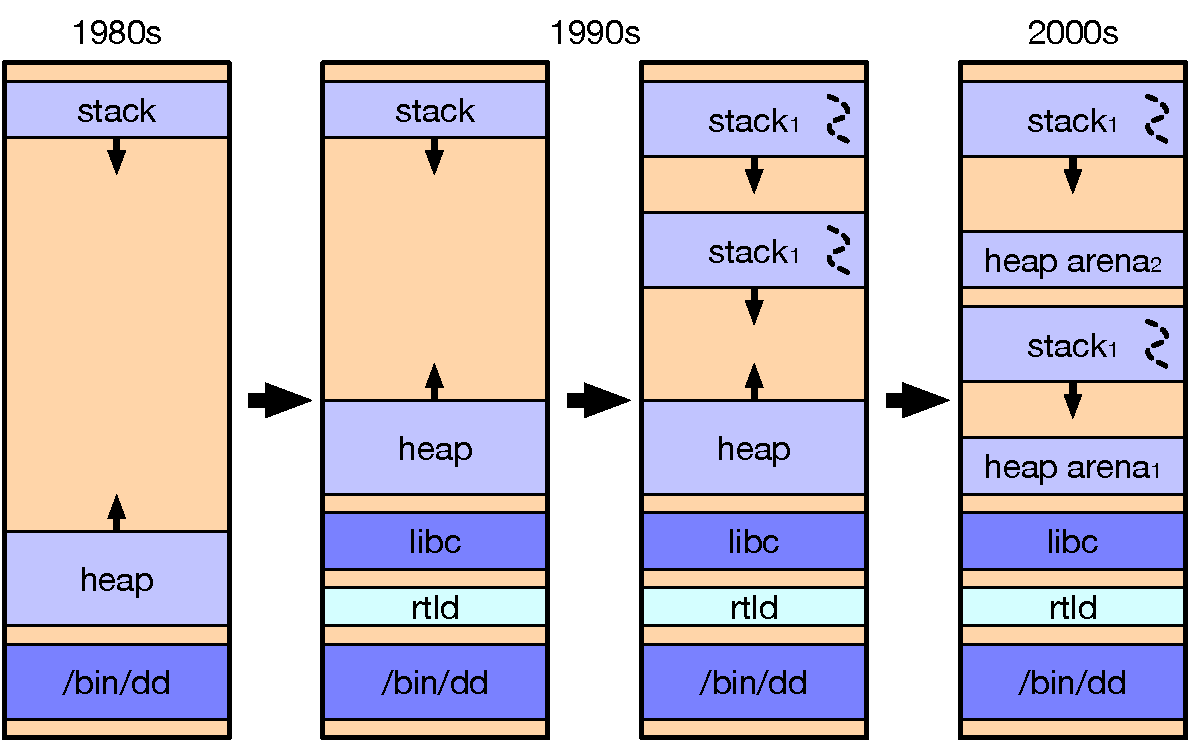
\includegraphics[width=1.1\textwidth]{../../figures/process-programmer-model.pdf}

    \column{0.45\textwidth}
      \begin{itemize}

	\pause

        \item 1980s: Code, heap, and stack

	\pause

        \item 1990s: Dynamic linking, multithreading

	\pause

        \item 2000s: Scalable memory allocators implement multiple
	  \textit{arenas}  (e.g., \texttt{jemalloc})

	\pause

        \item Coevolution with virtual memory research (Acetta, et al:
	  \textit{Mach} microkernel (1986); Navarro, et al \textit{Superpages}
	  (2002))
      \end{itemize}
  \end{columns}
\end{frame}

%\begin{frame}
%  \frametitle{Virtual memory (quick but painful primer)}
%
%  \begin{center}
%    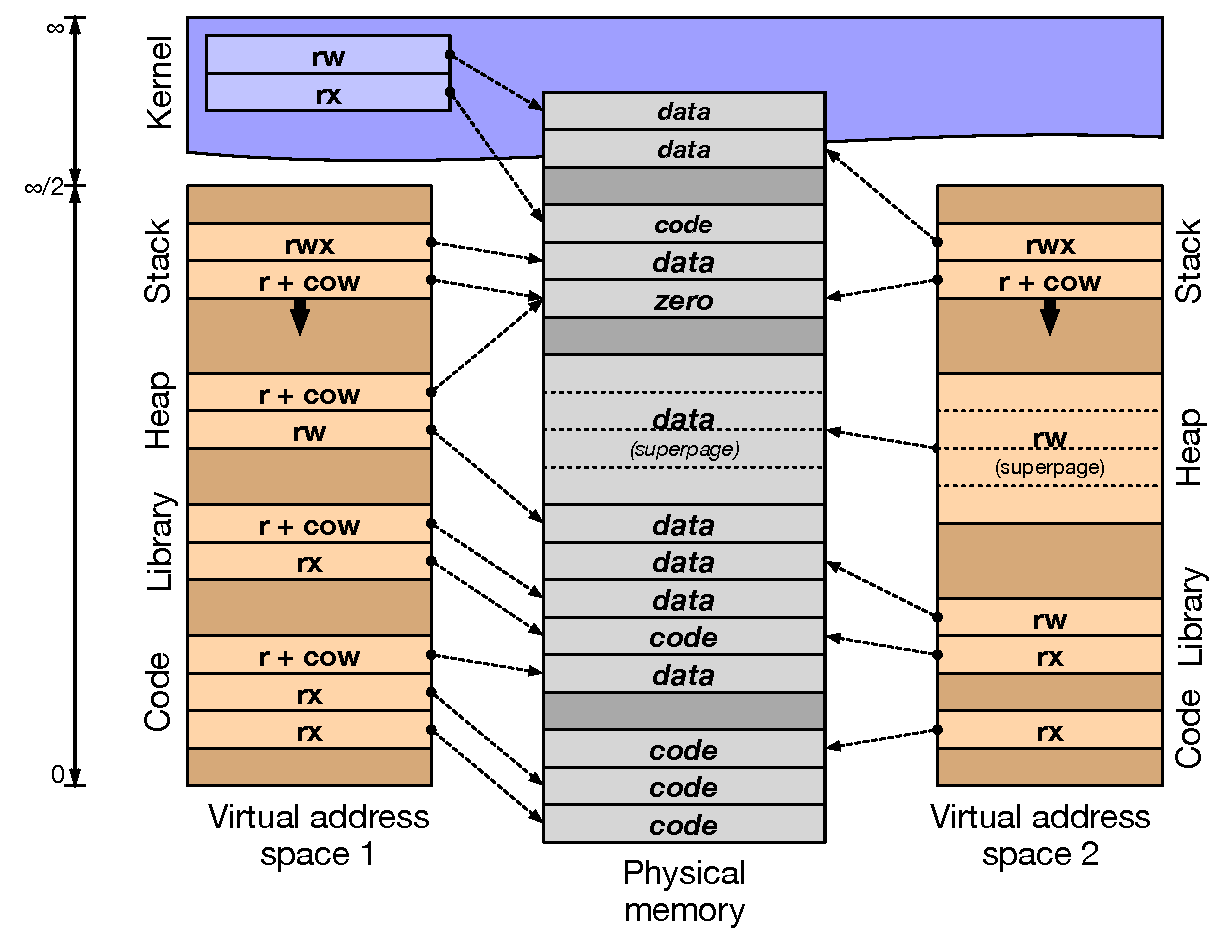
\includegraphics[width=0.8\textwidth]{../../figures/process-address-space.pdf}
%  \end{center}
%\end{frame}
%
%\begin{frame}
%  \frametitle{Virtual memory (quick but painful primer) (cont)}
%
%  \begin{itemize}
%    \item Memory Management Unit (MMU)
%    \begin{itemize}
%      \item Control available only to the supervisor
%      \item Mediates/transforms memory access (instruction fetch, load, store)
%      \item Trap fired on failure (e.g., permissions) to be handled by
%	software
%    \end{itemize}
%
%    \pause
%    \item Page tables
%    \begin{itemize}
%      \item Memory is laid out in \textit{pages} (4K)
%      \item OS-managed \textit{Page tables} map \textit{virtual pages}
%	into \textit{physical frames}
%      \item Access permissions, page attributes (e.g., caching)
%      \item Variable-size pages (now) supported
%    \end{itemize}
%
%    \pause
%    \item The Translation Look-aside Buffer (TLB)
%    \begin{itemize}
%      \item Hardware cache of entries -- avoid walking tables
%      \item Content Addressable Memory (CAM); 48? 1024? entries
%      \item TLB entry \textit{tagging}: entries \textit{global} or for a
%        specific process
%      \item Software- vs. hardware-managed
%    \end{itemize}
%
%%    \pause
%%
%%    \item Virtual address spaces
%%    \begin{itemize}
%%      \item Isolation vs. sharing
%%      \item BSS, \textit{Copy-on-Write}, \textit{Superpages}
%%    \end{itemize}
%
%    \pause
%
%    \item Hypervisors and I/O MMUs
%  \end{itemize}
%\end{frame}

\begin{frame}[fragile]
  \frametitle{Process address space: \texttt{dd}}

  \pause

  \begin{itemize}
    \item Inspect \texttt{dd} process address space with \texttt{procstat -v}.
  \end{itemize}

  \pause

  \begin{scriptsize}
\begin{verbatim}
root@beaglebone:/data # procstat -v 734
  PID      START        END PRT  RES PRES REF SHD FLAG TP PATH
  734     0x8000     0xd000 r-x    5    5   1   0 CN-- vn /bin/dd
  734    0x14000    0x16000 rw-    2    2   1   0 ---- df 
  734 0x20014000 0x20031000 r-x   29   32  31  14 CN-- vn /libexec/ld-elf.so.1
  734 0x20038000 0x20039000 rw-    1    0   1   0 C--- vn /libexec/ld-elf.so.1
  734 0x20039000 0x20052000 rw-   16   16   1   0 ---- df 
  734 0x20100000 0x2025f000 r-x  351  360  31  14 CN-- vn /lib/libc.so.7
  734 0x2025f000 0x20266000 ---    0    0   1   0 ---- df 
  734 0x20266000 0x2026e000 rw-    8    0   1   0 C--- vn /lib/libc.so.7
  734 0x2026e000 0x20285000 rw-    7  533   2   0 ---- df 
  734 0x20400000 0x20c00000 rw-  526  533   2   0 --S- df 
  734 0xbffe0000 0xc0000000 rwx    3    3   1   0 ---D df 
\end{verbatim}
  \end{scriptsize}

  \pause

  \begin{columns}[T]
      \column{0.35\textwidth}
        %Program binary, \\
	%Run-time linker, \\
	%Shared library, \\
	%BSS, Heap, Stack
      \column{0.25\textwidth}
	\texttt{r}: read \\
	\texttt{w}: write \\
	\texttt{x}: execute
      \column{0.375\textwidth}
        \texttt{C}: Copy-on-write \\
	\texttt{D}: Downward growth \\
	\texttt{S}: Superpage
  \end{columns}
\end{frame}

\begin{frame}[fragile]
  \frametitle{ELF binaries}

  \pause

  \begin{itemize}
    \item UNIX: Executable and Linkable Format (ELF)
    \item Mac OS X/iOS: Mach-O; Windows: PE/COFF; same ideas
    \item Inspect \texttt{dd} ELF program headers using \texttt{objdump -p}:
  \end{itemize}

  \pause

  \begin{scriptsize}
\begin{verbatim}
root@beaglebone:~ # objdump -p /bin/dd
/bin/dd:     file format elf32-littlearm
\end{verbatim}
  \end{scriptsize}

  \pause

  \begin{scriptsize}
\begin{verbatim}
Program Header:
0x70000001 off    0x0000469c vaddr 0x0000c69c paddr 0x0000c69c align 2**2
         filesz 0x00000158 memsz 0x00000158 flags r--
    PHDR off    0x00000034 vaddr 0x00008034 paddr 0x00008034 align 2**2
         filesz 0x000000e0 memsz 0x000000e0 flags r-x
  INTERP off    0x00000114 vaddr 0x00008114 paddr 0x00008114 align 2**0
         filesz 0x00000015 memsz 0x00000015 flags r--
    LOAD off    0x00000000 vaddr 0x00008000 paddr 0x00008000 align 2**15
         filesz 0x000047f8 memsz 0x000047f8 flags r-x
    LOAD off    0x000047f8 vaddr 0x000147f8 paddr 0x000147f8 align 2**15
         filesz 0x000001b8 memsz 0x00001020 flags rw-
 DYNAMIC off    0x00004804 vaddr 0x00014804 paddr 0x00014804 align 2**2
         filesz 0x000000f0 memsz 0x000000f0 flags rw-
    NOTE off    0x0000012c vaddr 0x0000812c paddr 0x0000812c align 2**2
         filesz 0x0000004c memsz 0x0000004c flags r--
\end{verbatim}
  \end{scriptsize}
\end{frame}

\begin{frame}
  \frametitle{Virtual memory (quick but painful primer)}

  \begin{center}
    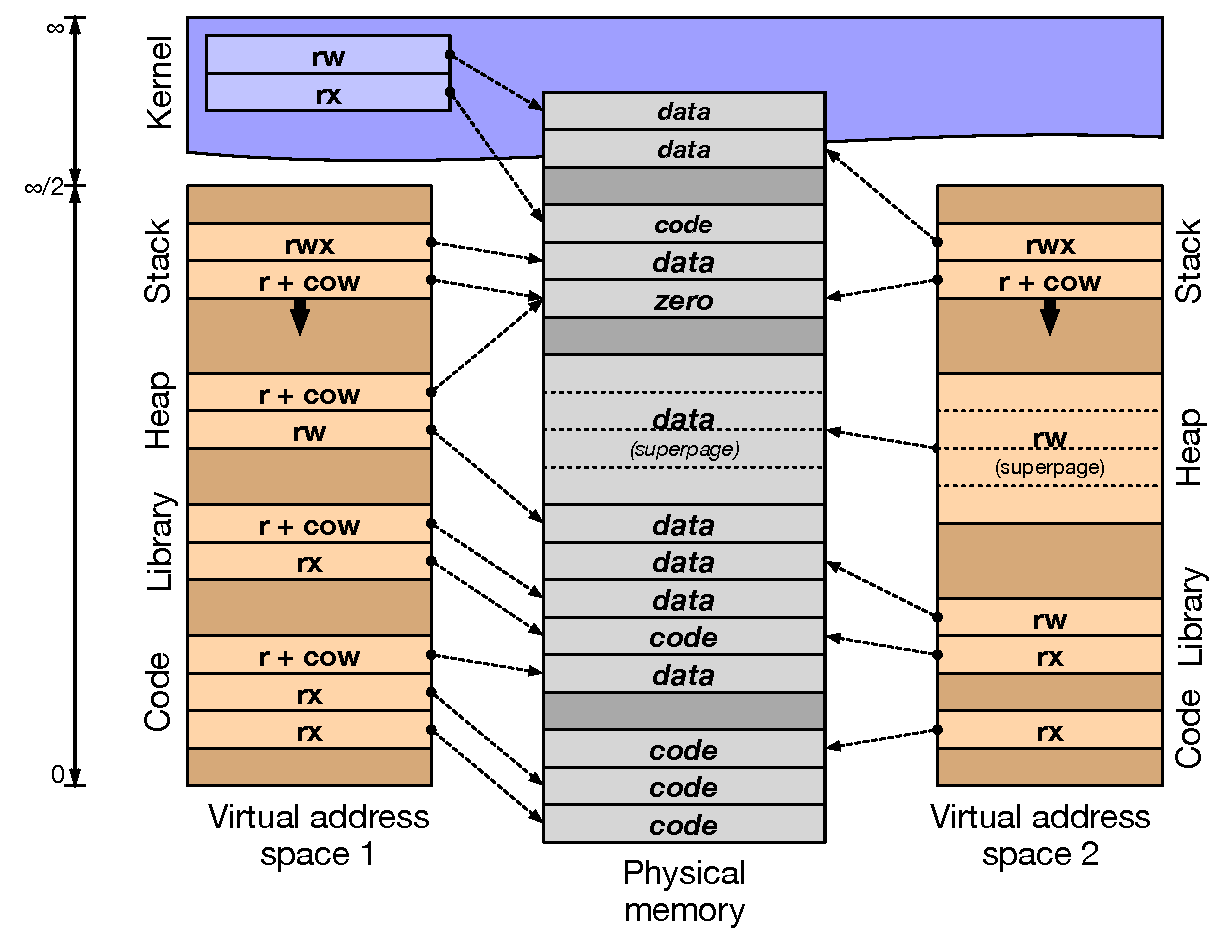
\includegraphics[width=0.8\textwidth]{../../figures/process-address-space.pdf}
  \end{center}
\end{frame}

\begin{frame}
  \frametitle{Virtual memory (quick but painful primer) (cont)}

  \begin{itemize}

    \pause

    \item Memory Management Unit (MMU)
    \begin{itemize}
      \item Transforms \textit{virtual addresses} into \textit{physical addresses}
      \item Memory is laid out in \textit{pages} (4K, 2M, 1G...)
      \item Control available only to the supervisor
      \item Software handles failures (e.g., permissions) via traps
    \end{itemize}

    \medskip
    \pause

    \item Page tables
    \begin{itemize}
      \item SW-managed \textit{page tables} provide \textit{virtual-physical
	mappings}
      \item Access permissions, page attributes (e.g., caching)
      \item Various configurations + traps implement BSS, COW, sharing, ...
    \end{itemize}

    \medskip
    \pause

    \item The Translation Look-aside Buffer (TLB)
    \begin{itemize}
      \item Hardware cache of entries -- avoid walking pagetables
      \item Content Addressable Memory (CAM); 48? 1024? entries
      \item TLB \textit{tags}: entries \textit{global} or for a specific process
      \item Software- vs. hardware-managed TLBs
    \end{itemize}

    \medskip
    \pause

%    \item Virtual address spaces
%    \begin{itemize}
%      \item Isolation vs. sharing
%      \item \textit{BSS}, \textit{Copy-on-Write}, \textit{Superpages}
%    \end{itemize}
%
%    \pause

    \item Hypervisors and \textit{I/O MMUs}: I/O sources as `processes'
  \end{itemize}
\end{frame}

\begin{frame}[fragile]
  \frametitle{Role of the run-time linker (\texttt{rtld})}

  \pause

  \begin{itemize}
    \item Static linking: program and libraries linked into a single binary

    \medskip
    \pause

    \item Dynamic linking: binary contains only the application, no libraries
    \begin{itemize}
      \item Shared libraries conserve memory by avoiding code duplication
      \item Program binaries contain a list of their \textit{library
	dependencies}
      \item The run-time linker (\texttt{rtld}) loads and links libraries
      \item Also used for plug-ins via \texttt{dlopen()}, \texttt{dlsym()}
    \end{itemize}

    \medskip
    \pause

    \item Three separate but related activities:
    \begin{itemize}
      \item \textit{Loading}: Load ELF segments at suitable virtual addresses
      \item \textit{Relocating}: Rewrite position-dependent code to load
	address
      \item \textit{Symbol resolution}: Rewrite inline addresses to other
	loaded code
    \end{itemize}
  \end{itemize}
\end{frame}

\begin{frame}[fragile]
  \frametitle{Role of the run-time linker (\texttt{rtld}) (cont)}

  \begin{scriptsize}
\begin{verbatim}
root@beaglebone:~ # ldd /bin/dd
/bin/dd:
        libc.so.7 => /lib/libc.so.7 (0x20100000)
\end{verbatim}
  \end{scriptsize}

  \begin{itemize}
    \item When the \texttt{execve} system call starts the new program:
    \begin{itemize}
      \item ELF binaries name their \textit{interpreter} in ELF metadata
      \item Kernel maps \texttt{rtld} and the application binary into memory
      \item Userspace execution in \texttt{rtld}
      \item \texttt{rtld} loads and links dynamic libraries, runs constructors
      \item \texttt{rtld} calls \texttt{main()}
    \end{itemize}

    \medskip
    \pause

    \item Optimisations:
    \begin{itemize}
      \item \textit{Lazy binding}: don't resolve all function symbols at load
	time
      \item \textit{Prelinking}: relocate, link in advance of execution
    \end{itemize}
  \end{itemize}
\end{frame}

\begin{frame}[fragile]
  \frametitle{Arguments and ELF auxiliary arguments}

  \pause

  \begin{itemize}
    \item C-program arguments are \texttt{argc}, \texttt{argv[]}, and
      \texttt{envv[]}:
  \end{itemize}

  \pause

  \begin{scriptsize}
\begin{verbatim}
root@beaglebone:/data # procstat -c 716
  PID COMM             ARGS                                                 
  716 dd               dd if=/dev/zero of=/dev/null bs=1m
\end{verbatim}
  \end{scriptsize}

  \pause

  \begin{itemize}
    \item The run-time linker also accepts arguments from the kernel:
  \end{itemize}

  \pause

  \begin{scriptsize}
\begin{verbatim}
root@beaglebone:/data # procstat -x 716
  PID COMM             AUXV             VALUE           
  716 dd               AT_PHDR          0x8034
  716 dd               AT_PHENT         32
  716 dd               AT_PHNUM         7
  716 dd               AT_PAGESZ        4096
  716 dd               AT_FLAGS         0
  716 dd               AT_ENTRY         0x8cc8
  716 dd               AT_BASE          0x20014000
  716 dd               AT_EXECPATH      0xbfffffc4
  716 dd               AT_OSRELDATE     1100062
  716 dd               AT_NCPUS         1
  716 dd               AT_PAGESIZES     0xbfffff9c
  716 dd               AT_PAGESIZESLEN  8
...
\end{verbatim}
  \end{scriptsize}
\end{frame}

\section{Trap to supervisor}

\begin{frame}
  \frametitle{Traps and system calls}

  \begin{itemize}
    \pause

    \item Asymmetric domain transition, \textit{trap}, shifts control to kernel
    \begin{itemize}
      \item \textit{Asynchronous traps}: e.g., timer, peripheral interrupts,
	Inter-Processor Interrupts (IPIs)
      \item \textit{Synchronous traps}: e.g., system calls, divide-by-zero,
	page faults
    \end{itemize}

    \pause
    \medskip

    \item \$pc to \textit{interrupt vector}: dedicated OS code to handle trap
    \item Key challenge: kernel must gain control safely, reliably, securely
    \begin{description}
      \item[RISC] \$pc saved, \$epc installed, control coprocessor (MMU, ...)
        made available, kernel memory access enabled, reserved exception 
        registers in ABI. \\
        Software must save other state (e.g., registers)
      \item[CISC] All that and: context saved to in-memory trap frame
    \end{description}

    \medskip
    \pause

  \item NB: User context switch = trap to kernel, restore a different context
  \end{itemize}
\end{frame}

\section{Conclusion}

\begin{frame}
  \frametitle{For next time}

  \begin{itemize}
    \item We will continue with system calls and traps
    \item Then more on virtual memory
    \item Threading models: the great debate

    \bigskip

    \item McKusick, et al: Chapter 6 (\textit{Memory Management})
    \item Optional: Anderson, et al, on \textit{Scheduler Activations}
  \end{itemize}

\end{frame}

\end{document}
